\begin{figure}[H]
	\center
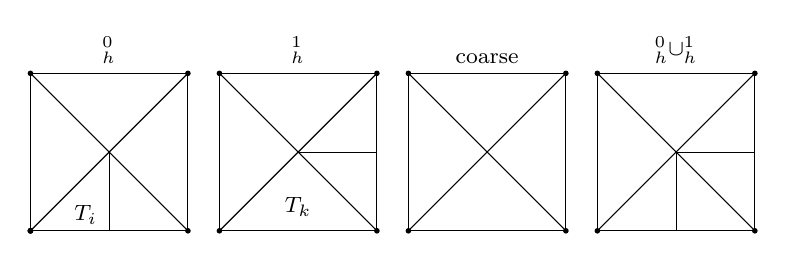
\begin{tikzpicture}[scale=2]
		
		\def \xone{0};
		\def \yone{0};		
		% first rectangle
		\coordinate (A) at (\xone,\yone);
		
        \draw (A) -- ++(0,1) -- ++(1,0)-- ++(0,-1) --cycle;
        \draw (A) -- ++(1,1);
        \draw (A) ++(0,1) -- ++(1,-1);
        \draw (A) ++(0.5,0) -- ++(0,0.5);
        \filldraw (A)         circle (0.4pt);
        \filldraw (A) ++(1,0) circle (0.4pt);
        \filldraw (A) ++(0,1) circle (0.4pt);
        \filldraw (A) ++(1,1) circle (0.4pt);
        
        
        % second rectangle
        \coordinate (A1) at (\xone + 1.2,\yone);
        
        \draw (A1) -- ++(0,1) -- ++(1,0)-- ++(0,-1) --cycle;
        \draw (A1) -- ++(1,1);
        \draw (A1) ++(0,1) -- ++(1,-1);
        \draw (A1) ++(0.5,0.5) -- ++(0.5,0);
        \filldraw (A)         circle (0.4pt);
        \filldraw (A1)         circle (0.4pt);
        \filldraw (A1) ++(1,0) circle (0.4pt);
        \filldraw (A1) ++(0,1) circle (0.4pt);
        \filldraw (A1) ++(1,1) circle (0.4pt);
        
        % third rectangle
        \coordinate (A2) at (\xone + 2.4,\yone);
        
        \draw (A2) -- ++(0,1) -- ++(1,0)-- ++(0,-1) --cycle;
        \draw (A2) -- ++(1,1);
        \draw (A2) ++(0,1) -- ++(1,-1);
        \filldraw (A)         circle (0.4pt);
        \filldraw (A2)         circle (0.4pt);
        \filldraw (A2) ++(1,0) circle (0.4pt);
        \filldraw (A2) ++(0,1) circle (0.4pt);
        \filldraw (A2) ++(1,1) circle (0.4pt);
        
        
        
        % forth rectangle
        \coordinate (A3) at (\xone + 3.6,\yone);
        
        \draw (A3) -- ++(0,1) -- ++(1,0)-- ++(0,-1) --cycle;
        \draw (A3) -- ++(1,1);
        \draw (A3) ++(0,1) -- ++(1,-1);
        \draw (A3) ++(0.5,0) -- ++(0,0.5);
        \draw (A3) ++(0.5,0.5) -- ++(0.5,0);
        \filldraw (A)         circle (0.4pt);
        \filldraw (A3)         circle (0.4pt);
        \filldraw (A3) ++(1,0) circle (0.4pt);
        \filldraw (A3) ++(0,1) circle (0.4pt);
        \filldraw (A3) ++(1,1) circle (0.4pt);
        
        \fill[black,font=\footnotesize] (A)  ++(0.5,1) node[above] {$\T^0_h$}
                                        (A1) ++(0.5,1) node[above] {$\T^1_h$}
                                        (A2) ++(0.5,1) node[above] {coarse}
                                        (A3) ++(0.5,1) node[above] {$\T^0_h \cup \T^1_h $}
                                        (A)  ++(0.35,0.1) node	   {$T_i$}
                                        (A1) ++(0.5,0.15)  node 	   {$T_k$} ;
\end{tikzpicture}

\caption{example of union of multiple meshes}
\label{ch_mult_union}
\end{figure}